\chapter{Revised Object-Oriented Structural Analysis Program}

\section{Introduction}
The object-oriented structural analysis program developed in Assignment 3 is extended in this work to incorporate thermal loading effects and support settlements. The original solver, based on the Direct Stiffness Method (DSM), supported linear static analysis of two-dimensional frame and truss structures using a modular and extensible class-based architecture.

The present revision introduces two additional capabilities that are essential in practical structural analysis. Thermal actions are incorporated to account for temperature-induced deformation and stress, while support settlements are modeled as prescribed displacements at restrained degrees of freedom. These extensions are implemented with minimal disruption to the existing solver, preserving its original architecture and workflow.

The objective of this chapter is to document the design modifications, implementation strategy, and theoretical integration of these new features within the existing object-oriented framework.

\pagebreak
\section{Analysis and Design Decisions}

\subsection{Thermal vs Settlement Modeling}

A key design decision was to treat thermal loading and support settlement as fundamentally different types of effects.

Thermal actions are internal to structural members and are therefore modeled at the element level using equivalent nodal loads derived from fixed-end forces. In contrast, support settlements represent imposed displacements at boundary conditions and must be incorporated at the global system level.

This distinction ensures that:

\begin{itemize}
    \item Thermal effects are handled locally within element formulations
    \item Settlement effects are handled globally through system partitioning
\end{itemize}

\subsection{Modification Strategy}

The solver was extended using the following approach:

\begin{itemize}
    \item The \texttt{Material} class was extended to include the coefficient of thermal expansion $\alpha$
    \item The \texttt{Section} class was extended to include section depth $d$ for thermal gradient calculations
    \item The \texttt{Node} class was extended to store prescribed displacements
    \item The \texttt{FrameElement} and \texttt{TrussElement} classes were extended to compute thermal fixed-end forces
    \item The \texttt{Structure} class was extended to solve the partitioned system for settlement
\end{itemize}

This approach preserved the original solver architecture while enabling the required functionality.

\pagebreak
\section{Revised UML and Class Modifications}

\subsection{Updated Class Responsibilities}

The primary modifications to the class structure are summarized below:

\begin{itemize}
    \item \textbf{Node:} Stores prescribed displacements for settlement modeling
    \item \textbf{Material:} Includes thermal expansion coefficient $\alpha$
    \item \textbf{Section:} Includes section depth $d$
    \item \textbf{FrameElement:} Computes thermal axial forces and bending moments
    \item \textbf{TrussElement:} Computes thermal axial forces only
    \item \textbf{Structure:} Handles partitioned system solution and reaction computation
\end{itemize}

\subsection{UML/Class Diagram}

\begin{figure}[H]
    \centering
  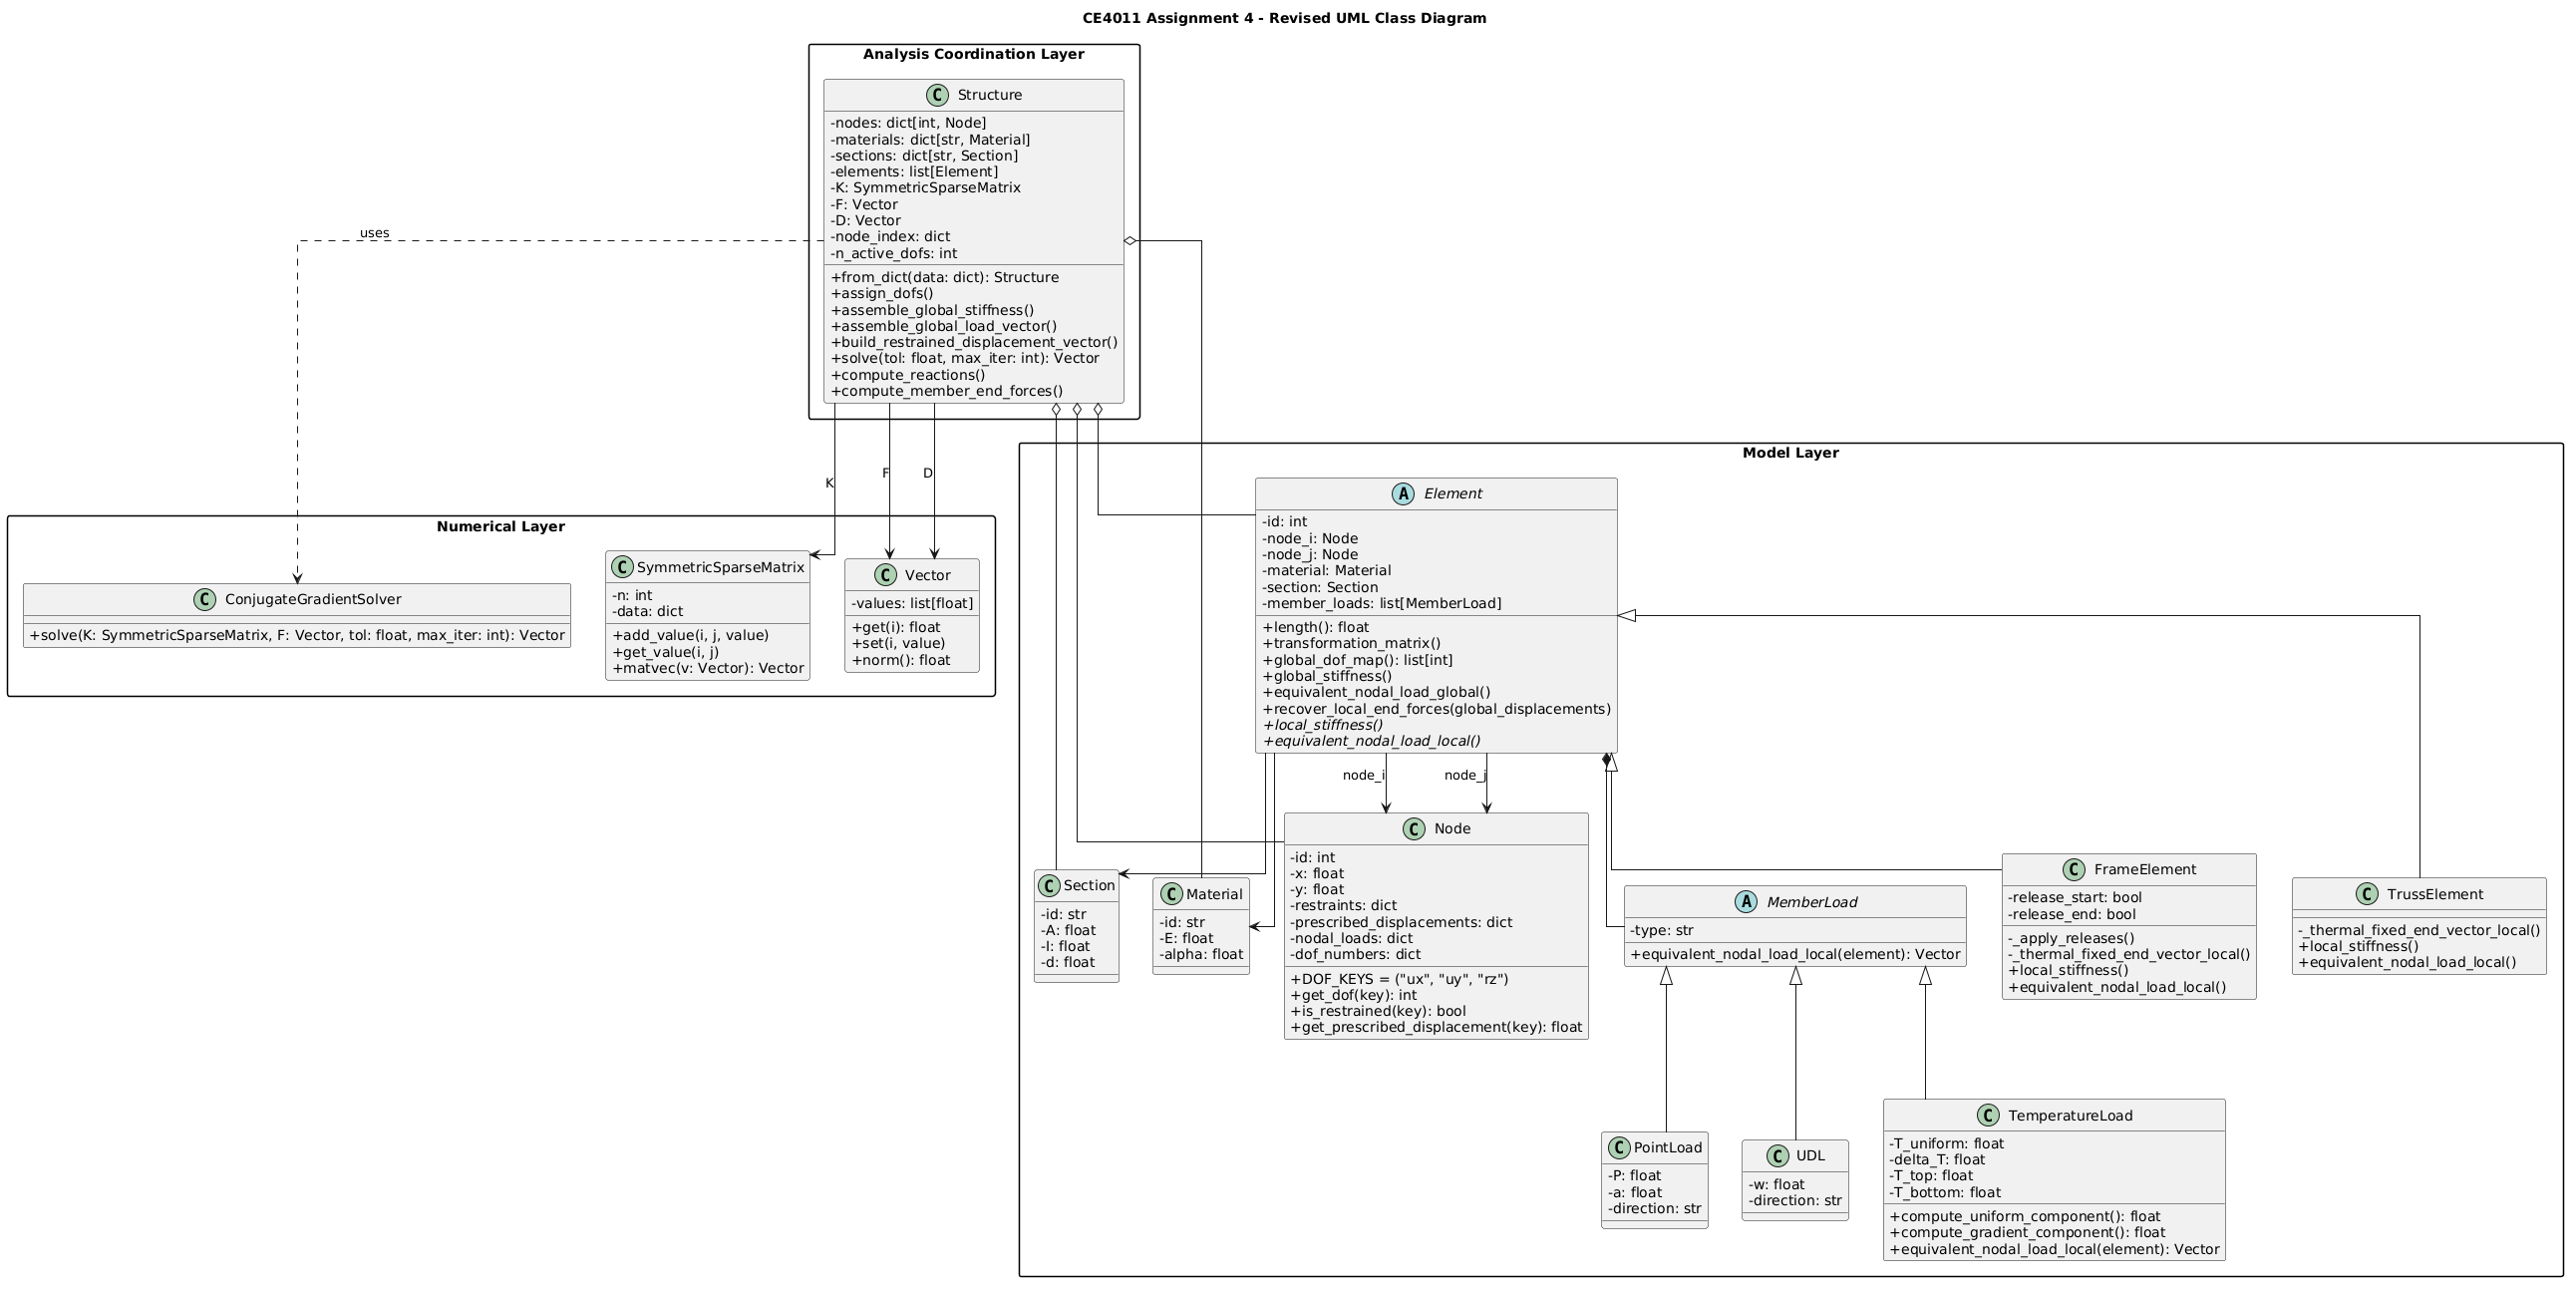
\includegraphics[width=0.95\textwidth]{UML_4.png}
    \caption{Revised UML/Class Diagram showing thermal and settlement extensions}
    \label{fig:uml_assignment4}
\end{figure}
\pagebreak
\section{Thermal Loading Extension}

\subsection{Modeling Approach}

Thermal effects are incorporated using the fixed-end force method. Temperature-induced strains are first computed and then converted into equivalent nodal forces acting on the structure. These forces are assembled into the global load vector without modifying the stiffness matrix.

\subsection{Uniform Temperature Change}

A uniform temperature change produces an axial strain:

\begin{equation}
\epsilon_{th} = \alpha \Delta T
\end{equation}

For a fully restrained member, this results in an axial force:

\begin{equation}
N_t = E A \alpha \Delta T
\end{equation}

This force is applied as an equivalent nodal load in the axial direction.

\subsection{Thermal Gradient Effects}

A temperature gradient across the section depth induces curvature:

\begin{equation}
\kappa = \alpha \frac{\Delta T}{d}
\end{equation}

The resulting bending moment is:

\begin{equation}
M_t = E I \alpha \frac{\Delta T}{d}
\end{equation}

This moment is represented as equivalent nodal moments at the element ends.

\subsection{Implementation in Elements}

Thermal loads are implemented by computing fixed-end force vectors within each element and converting them into equivalent nodal loads. For frame elements, both axial forces and bending moments are considered, while for truss elements only axial effects are included.
\pagebreak
\section{Support Settlement Extension}

\subsection{Settlement Modeling Approach}

Support settlements are modeled as prescribed displacements at restrained degrees of freedom. Unlike external loads, settlements modify the displacement boundary conditions and must be incorporated into the global system equations.

\subsection{Partitioned System Formulation}

The global stiffness equation is partitioned as:

\begin{equation}
\begin{bmatrix}
K_{ff} & K_{fr} \\
K_{rf} & K_{rr}
\end{bmatrix}
\begin{Bmatrix}
u_f \\
u_r
\end{Bmatrix}
=
\begin{Bmatrix}
F_f \\
F_r
\end{Bmatrix}
\end{equation}

For non-zero prescribed displacements, the system is solved as:

\begin{equation}
K_{ff} u_f = F_f - K_{fr} u_r
\end{equation}

Support reactions are obtained from:

\begin{equation}
F_r = K_{rf} u_f + K_{rr} u_r
\end{equation}

This formulation is implemented within the \texttt{Structure} class by constructing the restrained displacement vector and modifying the right-hand side of the system.
\pagebreak
\section{Updated Relationships and Workflow}

\subsection{Analysis Workflow}

The revised analysis procedure consists of the following steps:

\begin{enumerate}
    \item Assign degrees of freedom to all nodes
    \item Assemble the global stiffness matrix
    \item Assemble the global load vector including thermal loads
    \item Construct the restrained displacement vector for settlement
    \item Modify the right-hand side of the system
    \item Solve for unknown displacements
    \item Compute support reactions
    \item Recover member-end forces
\end{enumerate}

\subsection{Workflow Illustration}

\begin{figure}[H]
    \centering
    % \includegraphics[width=0.85\textwidth]{images/workflow_assignment4.png}
    \caption{Updated analysis workflow incorporating thermal and settlement effects}
    \label{fig:workflow_assignment4}
\end{figure}
\pagebreak
\section{Input Format}

\subsection{Data Schema Overview}

The solver accepts structured input defining nodes, materials, sections, elements, and loads. Thermal loads are specified as member loads, while settlements are defined as prescribed displacements at nodes.

\subsection{Example Input Snippet}

\begin{lstlisting}[language=Python,caption={Example thermal and settlement input},label={lst:input_snippet}]
{
  "elements": [
    {
      "type": "frame",
      "member_loads": [
        {"type": "thermal", "T_top": 50, "T_bottom": 0}
      ]
    }
  ],
  "prescribed_displacements": {
    "node_2": {"uy": -0.002}
  }
}
\end{lstlisting}
\pagebreak
\section{Output Format}

\subsection{Reported Quantities}

The solver produces the following outputs:

\begin{itemize}
    \item Nodal displacements
    \item Support reactions
    \item Member-end forces in local coordinates
\end{itemize}

\subsection{Output Table Structure}

\begin{table}[H]
    \centering
    \caption{Output quantities}
    \label{tab:output_quantities}
    \begin{tabular}{lll}
        \toprule
        Quantity & Unit & Description \\
        \midrule
        Displacement & m, rad & Nodal DOFs \\
        Reaction & N, Nm & Support forces and moments \\
        Member-end forces & N, Nm & Local element forces \\
        \bottomrule
    \end{tabular}
\end{table}
\pagebreak
\section{GitHub Repository Summary}

The complete implementation of the revised solver is available in the project repository.

The repository includes:
\begin{itemize}
    \item Core solver implementation (Assignment 3 and extensions)
    \item Thermal and settlement modules
    \item Unit and integration tests
    \item Example input cases
\end{itemize}

% TODO: Insert GitHub link
